\documentclass[11pt,a4paper]{article}
\usepackage[utf8]{inputenc}
\setlength{\textwidth}{18cm}
\setlength{\textheight}{26.7cm}
\setlength{\oddsidemargin}{-1.04cm}
\setlength{\evensidemargin}{-1.04cm}
\setlength{\topmargin}{-1.04cm}
\setlength{\headheight}{0pt}
\setlength{\headsep}{0pt}
\usepackage{amsmath}
\usepackage{tikz}
\usetikzlibrary{arrows.meta}
\pagestyle{empty}
\setlength{\parindent}{0pt}

\definecolor{colorpolo}{RGB}{242,35,66}
\definecolor{colorcero}{RGB}{0,151,69}
\definecolor{colorremocion}{RGB}{0,122,153}

\tikzset{
  eje/.style={black,line width=.8pt,-{Stealth[length=2mm]}},
  movimiento/.style={colorcero,line width=1.6pt,-{Stealth[length=2.4mm]}},
  permanencia/.style={colorpolo,line width=.8pt,-{Stealth[length=1.7mm]}},
  cancelado/.style={colorcero,dashed,line width=1.1pt},
  indicacion/.style={colorremocion,font=\sffamily\bfseries\small},
  inversion/.style={gray,font=\sffamily\scriptsize}
}

% Todos los puntos finitos se ubican segun x=1.6*sigma, con s=-sigma.
% Los valores escritos sobre los extremos son F(0) y F(infinito).
\newcommand{\fila}[6]{%
  % Altura comun: 0.34 cm por unidad del valor de la inmitancia.
  \pgfmathsetmacro{\alturaDC}{.34*(#5)}
  \pgfmathsetmacro{\alturaINF}{.34*(#6)}
  \draw[eje] (0,#2) -- (12.1,#2);
  % Marcadores T: el pie esta sobre el eje y la cabeza a la altura del valor.
  \draw[black,line width=1pt] (0,#2) -- (0,{#2+\alturaDC});
  \draw[black,line width=1pt] (-.15,{#2+\alturaDC}) -- (.15,{#2+\alturaDC});
  \draw[black,line width=1pt] (11.25,#2) -- (11.25,{#2+\alturaINF});
  \draw[black,line width=1pt] (11.10,{#2+\alturaINF}) -- (11.40,{#2+\alturaINF});
  \node[anchor=east,font=\Large] at (-.55,#2) {$#1$};
  \node[anchor=north,font=\small] at (0,{#2-.27}) {$0$};
  \node[anchor=south,font=\small] at (0,{#2+\alturaDC+.08}) {$#3$};
  \node[anchor=north,font=\small] at (11.25,{#2-.27}) {$\infty$};
  \node[anchor=south,font=\small] at (11.25,{#2+\alturaINF+.08}) {$#4$};
  \draw[gray,line width=.8pt] (10.10,{#2-.19}) -- (10.30,{#2+.19});
  \draw[gray,line width=.8pt] (10.26,{#2-.19}) -- (10.46,{#2+.19});
  \node[anchor=west,font=\small] at (12.20,#2) {$-\sigma$};
}

\newcommand{\polo}[3]{%
  \draw[colorpolo,line width=1.4pt]
    ({1.6*#1-.15},{#2-.15}) -- ({1.6*#1+.15},{#2+.15});
  \draw[colorpolo,line width=1.4pt]
    ({1.6*#1-.15},{#2+.15}) -- ({1.6*#1+.15},{#2-.15});
  \node[anchor=north,font=\small] at ({1.6*#1},{#2-.30}) {$#3$};
}

\newcommand{\cero}[3]{%
  \draw[colorcero,line width=1.4pt] ({1.6*#1},#2) circle (.205);
  \node[anchor=north,font=\small] at ({1.6*#1},{#2-.30}) {$#3$};
}

\newcommand{\rt}[2]{%
  \draw[colorremocion,line width=1.1pt] ({1.6*#1},#2) circle (.31);
  \node[indicacion,anchor=south] at ({1.6*#1},{#2+.37}) {RT};
}

\newcommand{\rp}[2]{%
  % Se rodea la T del valor en infinito, no un polo en infinito.
  \pgfmathsetmacro{\alturaRP}{.34*(#2)}
  \draw[colorremocion,line width=1.1pt]
    (11.25,{#1+\alturaRP/2}) ellipse (.32 and {\alturaRP/2+.10});
  \node[indicacion,anchor=south] at (11.25,{#1+\alturaRP+.60}) {RP};
}

\newcommand{\cancelacion}[2]{%
  \draw[cancelado] ({1.6*#1},#2) circle (.205);
}

\newcommand{\mueve}[4]{%
  \draw[movimiento] ({1.6*#1},{#2-1.00})
    to[out=-80,in=100] ({1.6*#3},{#4+.34});
}

\newcommand{\permanece}[3]{%
  \draw[permanencia] ({1.6*#1},{#2-1.00}) -- ({1.6*#1},{#3+.30});
}

\begin{document}
\begin{center}
  \begin{tikzpicture}[x=1cm,y=1cm]
    % 1. Impedancia inicial y remocion parcial de Z1=3/8 ohm.
    \fila{Z}{0}{\frac83}{1}{8/3}{1}
    \polo{1}{0}{1}
    \cero{2}{0}{2}
    \polo{3}{0}{3}
    \cero{4}{0}{4}
    \rp{0}{1}

    % 2. Z2 = 5/8 (s+11/5)(s+5) / ((s+1)(s+3)).
    \fila{Z_2}{-2.15}{\frac{55}{24}}{\frac58}{55/24}{5/8}
    \polo{1}{-2.15}{1}
    \cero{2.2}{-2.15}{\frac{11}{5}}
    \polo{3}{-2.15}{3}
    \cero{5}{-2.15}{5}
    \mueve{2}{0}{2.2}{-2.15}
    \mueve{4}{0}{5}{-2.15}
    \permanece{1}{0}{-2.15}
    \permanece{3}{0}{-2.15}

    % 3. Inversion: los polos y ceros intercambian su naturaleza.
    \fila{Y_2}{-4.30}{\frac{24}{55}}{\frac85}{24/55}{8/5}
    \cero{1}{-4.30}{1}
    \polo{2.2}{-4.30}{\frac{11}{5}}
    \cero{3}{-4.30}{3}
    \polo{5}{-4.30}{5}
    \rt{5}{-4.30}

    % 4. Remocion total de la admitancia RC: (32/35) s/(s+5).
    % El polo -5 y el cero desplazado hasta -5 se cancelan.
    \fila{Y_4}{-6.45}{\frac{24}{55}}{\frac{24}{35}}{24/55}{24/35}
    \cero{1.4}{-6.45}{\frac75}
    \polo{2.2}{-6.45}{\frac{11}{5}}
    \cancelacion{5}{-6.45}
    \mueve{1}{-4.30}{1.4}{-6.45}
    \mueve{3}{-4.30}{5}{-6.45}
    \permanece{2.2}{-4.30}{-6.45}

    % 5. Inversion y remocion parcial de Z2=105/104 ohm.
    \fila{Z_4}{-8.60}{\frac{55}{24}}{\frac{35}{24}}{55/24}{35/24}
    \polo{1.4}{-8.60}{\frac75}
    \cero{2.2}{-8.60}{\frac{11}{5}}
    \rp{-8.60}{35/24}

    % 6. Z6 = 35/78 (s+4)/(s+7/5).
    \fila{Z_6}{-10.75}{\frac{50}{39}}{\frac{35}{78}}{50/39}{35/78}
    \polo{1.4}{-10.75}{\frac75}
    \cero{4}{-10.75}{4}
    \mueve{2.2}{-8.60}{4}{-10.75}
    \permanece{1.4}{-8.60}{-10.75}

    % 7. Inversion y remocion total de (507/350) s/(s+4).
    \fila{Y_6}{-12.90}{\frac{39}{50}}{\frac{78}{35}}{39/50}{78/35}
    \cero{1.4}{-12.90}{\frac75}
    \polo{4}{-12.90}{4}
    \rt{4}{-12.90}

    % 8. El cero llega al polo -4: queda una conductancia constante.
    \fila{Y_8}{-15.05}{\frac{39}{50}}{\frac{39}{50}}{39/50}{39/50}
    \cancelacion{4}{-15.05}
    \mueve{1.4}{-12.90}{4}{-15.05}

    % 9. Ultima resistencia, Z3 = 1/Y8 = 50/39 ohm.
    \fila{Z_8}{-17.20}{\frac{50}{39}}{\frac{50}{39}}{50/39}{50/39}
  \end{tikzpicture}
\end{center}
\end{document}
